\documentclass[12pt]{article}\usepackage[]{graphicx}\usepackage[]{color}
%% maxwidth is the original width if it is less than linewidth
%% otherwise use linewidth (to make sure the graphics do not exceed the margin)
\makeatletter
\def\maxwidth{ %
  \ifdim\Gin@nat@width>\linewidth
    \linewidth
  \else
    \Gin@nat@width
  \fi
}
\makeatother

\definecolor{fgcolor}{rgb}{0.345, 0.345, 0.345}
\newcommand{\hlnum}[1]{\textcolor[rgb]{0.686,0.059,0.569}{#1}}%
\newcommand{\hlstr}[1]{\textcolor[rgb]{0.192,0.494,0.8}{#1}}%
\newcommand{\hlcom}[1]{\textcolor[rgb]{0.678,0.584,0.686}{\textit{#1}}}%
\newcommand{\hlopt}[1]{\textcolor[rgb]{0,0,0}{#1}}%
\newcommand{\hlstd}[1]{\textcolor[rgb]{0.345,0.345,0.345}{#1}}%
\newcommand{\hlkwa}[1]{\textcolor[rgb]{0.161,0.373,0.58}{\textbf{#1}}}%
\newcommand{\hlkwb}[1]{\textcolor[rgb]{0.69,0.353,0.396}{#1}}%
\newcommand{\hlkwc}[1]{\textcolor[rgb]{0.333,0.667,0.333}{#1}}%
\newcommand{\hlkwd}[1]{\textcolor[rgb]{0.737,0.353,0.396}{\textbf{#1}}}%

\usepackage{framed}
\makeatletter
\newenvironment{kframe}{%
 \def\at@end@of@kframe{}%
 \ifinner\ifhmode%
  \def\at@end@of@kframe{\end{minipage}}%
  \begin{minipage}{\columnwidth}%
 \fi\fi%
 \def\FrameCommand##1{\hskip\@totalleftmargin \hskip-\fboxsep
 \colorbox{shadecolor}{##1}\hskip-\fboxsep
     % There is no \\@totalrightmargin, so:
     \hskip-\linewidth \hskip-\@totalleftmargin \hskip\columnwidth}%
 \MakeFramed {\advance\hsize-\width
   \@totalleftmargin\z@ \linewidth\hsize
   \@setminipage}}%
 {\par\unskip\endMakeFramed%
 \at@end@of@kframe}
\makeatother

\definecolor{shadecolor}{rgb}{.97, .97, .97}
\definecolor{messagecolor}{rgb}{0, 0, 0}
\definecolor{warningcolor}{rgb}{1, 0, 1}
\definecolor{errorcolor}{rgb}{1, 0, 0}
\newenvironment{knitrout}{}{} % an empty environment to be redefined in TeX

\usepackage{alltt}
% !Rnw weave = knitr
%
%\makeatletter
% \VignetteIndexEntry{Comparison of response functions}
% \VignetteEngine{knitr}
%\makeatother
%

%\usepackage{url}
\usepackage[T1]{fontenc}
\usepackage[utf8]{inputenc}
\usepackage{fancyvrb}
\usepackage[pdfborder={0 0 0}]{hyperref}
\usepackage{bookmark}
\usepackage{url}
\usepackage{upquote}
\usepackage{graphicx}
\usepackage{grffile}
\usepackage{float}
\usepackage{natbib}
\usepackage{amsmath}
\usepackage{amssymb}
\usepackage{hyperref}
\usepackage{geometry}
\geometry{verbose,tmargin=3cm,bmargin=5cm,lmargin=2.5cm,rmargin=2.5cm}
\usepackage[font=sf, labelfont={sf,bf}, margin=2cm]{caption}
\usepackage{color}
\raggedright
%
\author{Andrew J. Barbour}
\title{Comparison of response functions in \kit{}}
%
\IfFileExists{upquote.sty}{\usepackage{upquote}}{}
\begin{document}
%
\newcommand{\SC}[1]{\textsc{#1}}
\newcommand{\Rcmd}[1]{\texttt{#1}}
\newcommand{\kit}[0]{\href{http://abarbour.github.io/kitagawa/}{\color{blue}\Rcmd{kitagawa}}}
\newcommand{\bidxa}[1]{\index{#1}{\textbf{#1}}} 
\newcommand{\bidxb}[2]{\index{#2}{\textbf{#1}}} 
\newcommand{\idxa}[1]{\index{#1}{#1}} 
\newcommand{\idxb}[2]{\index{#2}{#1}} 
%
\maketitle
%
\begin{abstract}
In this vignette I demonstrate the response functions found in 
the package
\kit{}, which are appropriate for modeling the effect of
harmonic volumetric strain or pressure-head fluctuations in
sealed and open water wells.
There is only one sealed-well response function, from
\citet{kitagawa2011}, and this gives the complex frequency response of
virtual water height $Z$ or pressure $P$ as a function of
areal %volumetric?
strain $\epsilon$.
There is a suite of open-well response functions, from 
\citet{cooper1965, hsieh1987, rojstaczer1988, liu1989}; and
these give the complex frequency response of
water height as a function of aquifer head $H$ or pressure.
\end{abstract}
%
\tableofcontents

\clearpage
\section{Introduction}

 The underlying physical model of these response functions
 is based upon the assumption that fluid flows radially
 through an homogeneous, isotropic, confined aquifer.
%
 The underlying principle is as follows.  When a harmonic wave induces
 strain in a confined aquifer (one having aquitards above and below it), 
 fluid flows radially into, and out of a well penetrating the aquifer.
 The flow-induced drawdown, $s$, is governed by the following 
 partial differential equation, expressed in radial coordinates($r$):
\begin{equation}
 \frac{\partial^2 s}{\partial r^2} + \frac{1}{r} 
 \frac{\partial s}{ \partial r} - \frac{S}{T}\frac{\partial s}{\partial t} = 0
\end{equation}
 where $S$ and $T$ are the aquifer storativity and transmissivity respectively.
 
 The solution to this PDE, with periodic discharge boundary conditions,
 gives the amplitude and phase response we wish to calculate.
 The solution  for an open well was first presented by
 \citet{cooper1965}, and subsequently modified by \citet{rojstaczer1988, liu1989}.
 \citet{kitagawa2011} adapted the solution
 of \citet{hsieh1987} for the case of a sealed well.
 
 These models are applicable to any quasi-static process involving harmonic, 
 volumetric strain of an aquifer 
 (e.g., passing Rayleigh waves, or changes in the Earth's tidal potential). 
 In practice, however, the presence of permeable fractures can violate the
 assumption of isotropic permeability, which may substantially
 alter the response by introducing shear-strain coupling. Such
 complications are beyond the scope of these models.

\section{Preliminaries}


%opts_knit$set(verbose = TRUE)

Load the necessary packages:

\begin{knitrout}\small
\definecolor{shadecolor}{rgb}{0.969, 0.969, 0.969}\color{fgcolor}\begin{kframe}
\begin{alltt}
\hlkwd{library}\hlstd{(RColorBrewer)}
\hlstd{Set1} \hlkwb{<-} \hlkwd{brewer.pal}\hlstd{(}\hlnum{8}\hlstd{,} \hlstr{"Set1"}\hlstd{)}
\hlkwd{library}\hlstd{(signal,} \hlkwc{warn.conflicts} \hlstd{=} \hlnum{FALSE}\hlstd{)}
\hlkwd{library}\hlstd{(kitagawa)}
\end{alltt}


{\ttfamily\noindent\itshape\color{messagecolor}{\#\# Loaded kitagawa (2.2.0) -- Spectral response of water wells}}\end{kframe}
\end{knitrout}

Setup some constants:

\begin{knitrout}\small
\definecolor{shadecolor}{rgb}{0.969, 0.969, 0.969}\color{fgcolor}\begin{kframe}
\begin{alltt}
\hlstd{S.} \hlkwb{<-} \hlnum{1e-05}  \hlcom{# Storativity [nondimensional]}
\hlstd{T.} \hlkwb{<-} \hlnum{1e-04}  \hlcom{# Transmissivity [m**2 / s]}
\hlstd{D.} \hlkwb{<-} \hlstd{T.}\hlopt{/}\hlstd{S.}  \hlcom{# Diffusivity [m**2 / s]}
\hlstd{Ta} \hlkwb{<-} \hlnum{50}  \hlcom{# Aquifer thickness [m] #100}
\hlstd{Hw} \hlkwb{<-} \hlstd{z} \hlkwb{<-} \hlnum{50}  \hlcom{# Depth to water table [m] #10}

\hlcom{# Using ANO1 stats from Kit Tbl 1}
\hlstd{Rc.} \hlkwb{<-} \hlnum{0.075}  \hlcom{# Radius of cased portion of well [m]}
\hlstd{Lc.} \hlkwb{<-} \hlnum{570}  \hlcom{# Length of cased portion of well [m]}
\hlstd{Rs.} \hlkwb{<-} \hlnum{0.135}  \hlcom{# Radius of screened portion of well [m]}
\hlstd{Ls.} \hlkwb{<-} \hlnum{15}  \hlcom{# Length of screened portion of well [m]}
\hlstd{Vw.} \hlkwb{<-} \hlkwd{sensing_volume}\hlstd{(Rc., Lc., Rs., Ls.)}  \hlcom{# volume of fluid [m**3]}
\hlcom{# parameters assumed by well_response: rho=1000 # density of rock}
\hlcom{# [kg/m**3] Kf=2.2e9 # Bulk modulus of fluid [Pascals] grav=9.81 #}
\hlcom{# gravitational acceleration [m/s**2]}
\hlstd{rhog} \hlkwb{<-} \hlnum{9.81} \hlopt{*} \hlnum{1000}
\hlcom{# Kitagawa Fig 7: Ku B / Kw Aw = 3 => Aw==4.8 at 40GPa}
\hlstd{Ku.} \hlkwb{<-} \hlnum{4e+10}  \hlcom{# Bulk modulus [Pascals]}
\hlstd{B.} \hlkwb{<-} \hlnum{0.5}  \hlcom{# Skemptons ratio [nondimensional]}
\end{alltt}
\end{kframe}
\end{knitrout}

And create the dimensionless frequencies, 
defined by $z^2 \omega / 2 D$,
where $D$ is the hydraulic diffusivity:

\begin{knitrout}\small
\definecolor{shadecolor}{rgb}{0.969, 0.969, 0.969}\color{fgcolor}\begin{kframe}
\begin{alltt}
\hlcom{# Frequencies}
\hlstd{Q} \hlkwb{<-} \hlnum{10}\hlopt{^}\hlkwd{seq}\hlstd{(}\hlopt{-}\hlnum{5}\hlstd{,} \hlnum{2}\hlstd{,} \hlkwc{by} \hlstd{=} \hlnum{0.05}\hlstd{)}  \hlcom{# [nondimensional]}
\hlstd{lQ} \hlkwb{<-} \hlkwd{log10}\hlstd{(Q)}
\hlstd{omega} \hlkwb{<-} \hlkwd{omega_norm}\hlstd{(Q, z, D.,} \hlkwc{invert} \hlstd{=} \hlnum{TRUE}\hlstd{)}  \hlcom{# [Hz]}

\hlstd{Phase} \hlkwb{<-} \hlkwa{function}\hlstd{(}\hlkwc{Z}\hlstd{) \{}
    \hlstd{Phs.} \hlkwb{<-} \hlkwd{Arg}\hlstd{(Z)}  \hlcom{# will wrap to -pi/pi}
    \hlstd{uPhs.} \hlkwb{<-} \hlstd{signal}\hlopt{::}\hlkwd{unwrap}\hlstd{(Phs.,} \hlkwc{tol} \hlstd{= pi}\hlopt{/}\hlnum{30}\hlstd{)}
    \hlkwd{return}\hlstd{(}\hlkwd{data.frame}\hlstd{(}\hlkwc{Phs} \hlstd{= Phs.,} \hlkwc{uPhs} \hlstd{= uPhs.))}
\hlstd{\}}

\hlcom{# Responses converted to pressure if TRUE}
\hlstd{asP} \hlkwb{<-} \hlnum{FALSE}
\hlstd{ZasP} \hlkwb{<-} \hlnum{FALSE}
\end{alltt}
\end{kframe}
\end{knitrout}

And onto the response functions...

\clearpage
\section{Sealed well response}

\subsection{Strain: Kitagawa et al. (2011)}
%
\begin{knitrout}\small
\definecolor{shadecolor}{rgb}{0.969, 0.969, 0.969}\color{fgcolor}\begin{kframe}
\begin{alltt}
\hlstd{wrsp} \hlkwb{<-} \hlkwd{well_response}\hlstd{(omega,} \hlkwc{T.} \hlstd{= T.,} \hlkwc{S.} \hlstd{= S.,} \hlkwc{Vw.} \hlstd{= Vw.,} \hlkwc{Rs.} \hlstd{= Rs.,} \hlkwc{Ku.} \hlstd{= Ku.,}
    \hlkwc{B.} \hlstd{= B.,} \hlkwc{Avs} \hlstd{=} \hlnum{1}\hlstd{,} \hlkwc{Aw} \hlstd{=} \hlnum{1}\hlstd{,} \hlkwc{as.pressure} \hlstd{= asP)}
\hlkwd{plot}\hlstd{(wrsp)}  \hlcom{# uses plot.wrsp method}
\end{alltt}
\end{kframe}
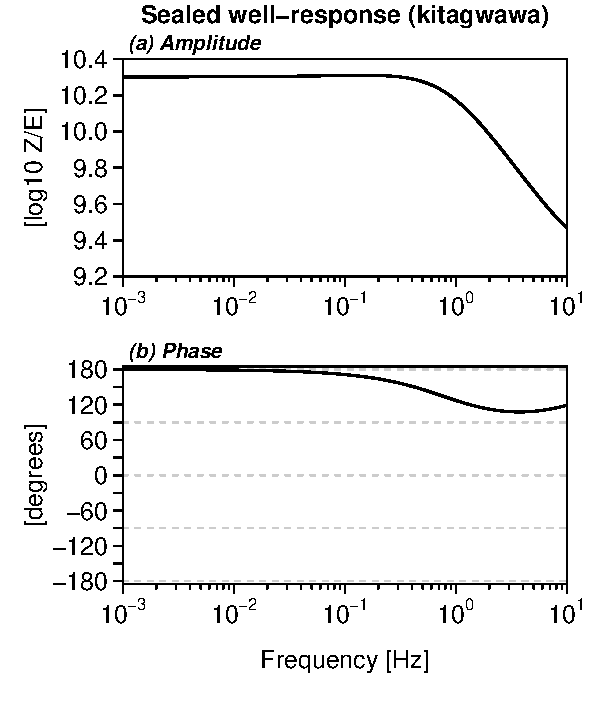
\includegraphics[width=\maxwidth]{figure/KITRESP-1} 
\begin{kframe}\begin{alltt}
\hlstd{crsp} \hlkwb{<-} \hlstd{wrsp[[}\hlstr{"Response"}\hlstd{]][,} \hlnum{2}\hlstd{]}  \hlcom{# Complex response}
\hlstd{kGain} \hlkwb{<-} \hlkwd{Mod}\hlstd{(crsp)}\hlopt{/}\hlstd{Ku.}\hlopt{/}\hlstd{B.}  \hlcom{# Amplitude (or Gain)}
\hlstd{kP} \hlkwb{<-} \hlkwd{Phase}\hlstd{(crsp)}  \hlcom{# Phase}
\end{alltt}
\end{kframe}
\end{knitrout}

\begin{figure}[htb!]
\begin{center}
\begin{knitrout}\small
\definecolor{shadecolor}{rgb}{0.969, 0.969, 0.969}\color{fgcolor}
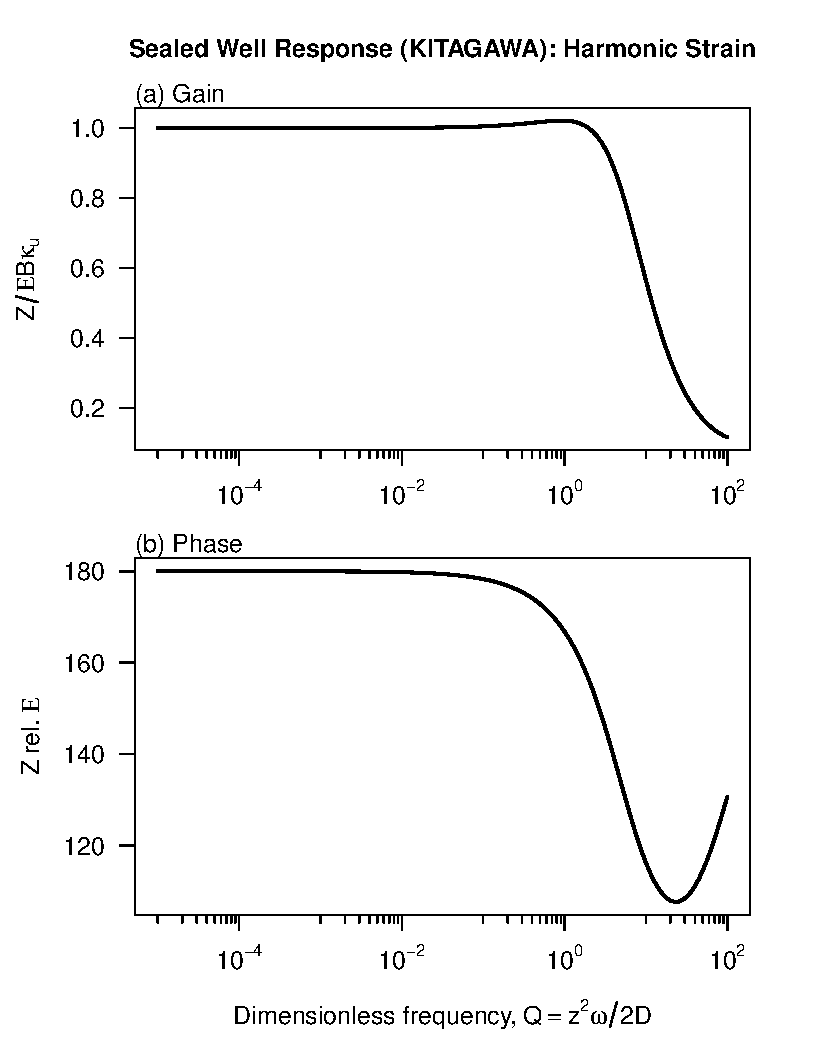
\includegraphics[width=\maxwidth]{figure/KITRESPFIG-1} 

\end{knitrout}
\caption{The response of a sealed well to harmonic areal strain using
the Kitagawa model. The amplitude is normalized by Skempton's coefficient $B$
and the undrained bulk modulus $\kappa_u$.
Frequency is dimensionless, based on the well-depth $z$ and the diffusivity $D$.
}
\label{fig:wrsp}
\end{center}
\end{figure}

\clearpage
\section{Open well response}

\subsection{Pressure head: Cooper et al. (1965)}

\begin{knitrout}\small
\definecolor{shadecolor}{rgb}{0.969, 0.969, 0.969}\color{fgcolor}\begin{kframe}
\begin{alltt}
\hlstd{wrsp} \hlkwb{<-} \hlkwd{open_well_response}\hlstd{(omega,} \hlkwc{T.} \hlstd{= T.,} \hlkwc{S.} \hlstd{= S.,} \hlkwc{Ta} \hlstd{= Ta,} \hlkwc{Hw} \hlstd{= Hw,}
    \hlkwc{model} \hlstd{=} \hlstr{"cooper"}\hlstd{,} \hlkwc{as.pressure} \hlstd{= ZasP)}
\hlkwd{plot}\hlstd{(wrsp)}
\end{alltt}
\end{kframe}
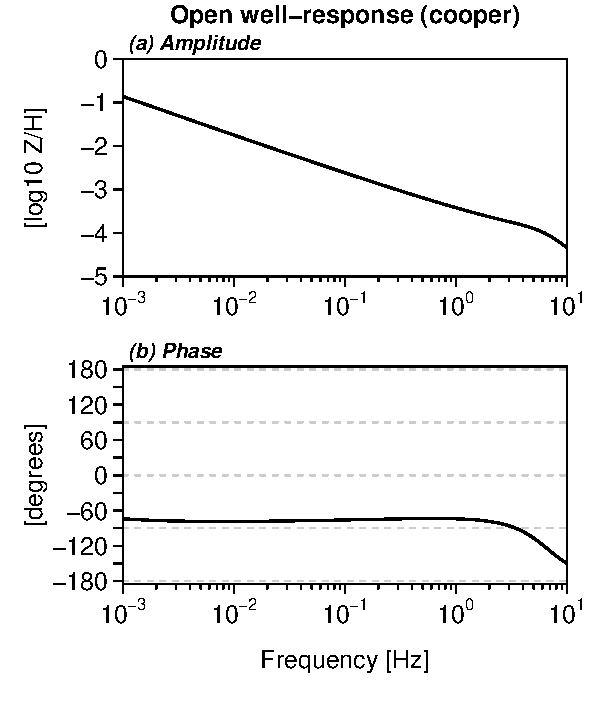
\includegraphics[width=\maxwidth]{figure/COOPERRESP-1} 
\begin{kframe}\begin{alltt}
\hlstd{crsp} \hlkwb{<-} \hlstd{wrsp[[}\hlstr{"Response"}\hlstd{]][,} \hlnum{2}\hlstd{]}
\hlstd{cGain} \hlkwb{<-} \hlkwd{Mod}\hlstd{(crsp)}
\hlstd{cP} \hlkwb{<-} \hlkwd{Phase}\hlstd{(crsp)}
\end{alltt}
\end{kframe}
\end{knitrout}

\begin{figure}[htb!]
\begin{center}
\begin{knitrout}\small
\definecolor{shadecolor}{rgb}{0.969, 0.969, 0.969}\color{fgcolor}
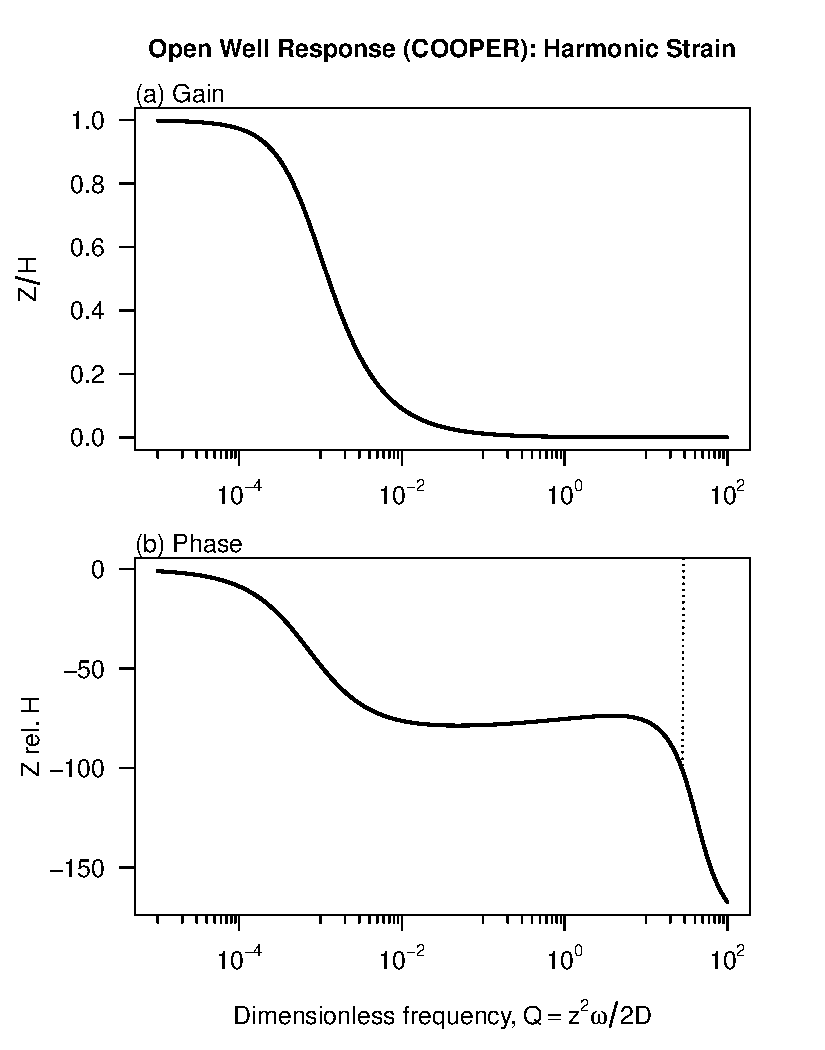
\includegraphics[width=\maxwidth]{figure/COOPERRESPFIG-1} 

\end{knitrout}
\caption{The response of an open well to harmonic areal strain using
the Cooper model. 
Frequency is dimensionless, based on the well-depth $z$ and the diffusivity $D$.
}
\label{fig:owrsp-coop}
\end{center}
\end{figure}

\clearpage
\subsection{Pressure head: Hsieh et al. (1987)}

\begin{knitrout}\small
\definecolor{shadecolor}{rgb}{0.969, 0.969, 0.969}\color{fgcolor}\begin{kframe}
\begin{alltt}
\hlstd{wrsp} \hlkwb{<-} \hlkwd{open_well_response}\hlstd{(omega,} \hlkwc{T.} \hlstd{= T.,} \hlkwc{S.} \hlstd{= S.,} \hlkwc{Ta} \hlstd{= Ta,} \hlkwc{Hw} \hlstd{= Hw,}
    \hlkwc{model} \hlstd{=} \hlstr{"hsieh"}\hlstd{,} \hlkwc{as.pressure} \hlstd{= ZasP)}
\hlkwd{plot}\hlstd{(wrsp)}
\end{alltt}
\end{kframe}
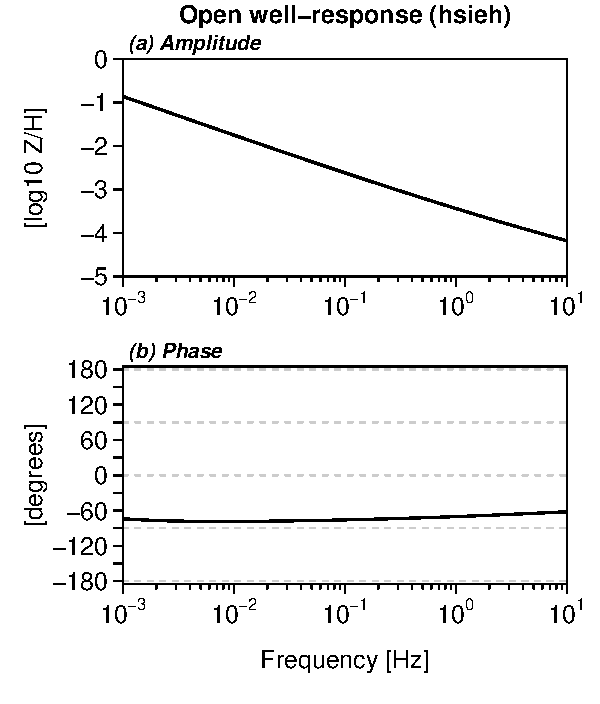
\includegraphics[width=\maxwidth]{figure/HSIEHRESP-1} 
\begin{kframe}\begin{alltt}
\hlstd{crsp} \hlkwb{<-} \hlstd{wrsp[[}\hlstr{"Response"}\hlstd{]][,} \hlnum{2}\hlstd{]}
\hlstd{hGain} \hlkwb{<-} \hlkwd{Mod}\hlstd{(crsp)}
\hlstd{hP} \hlkwb{<-} \hlkwd{Phase}\hlstd{(crsp)}
\end{alltt}
\end{kframe}
\end{knitrout}

\begin{figure}[htb!]
\begin{center}
\begin{knitrout}\small
\definecolor{shadecolor}{rgb}{0.969, 0.969, 0.969}\color{fgcolor}
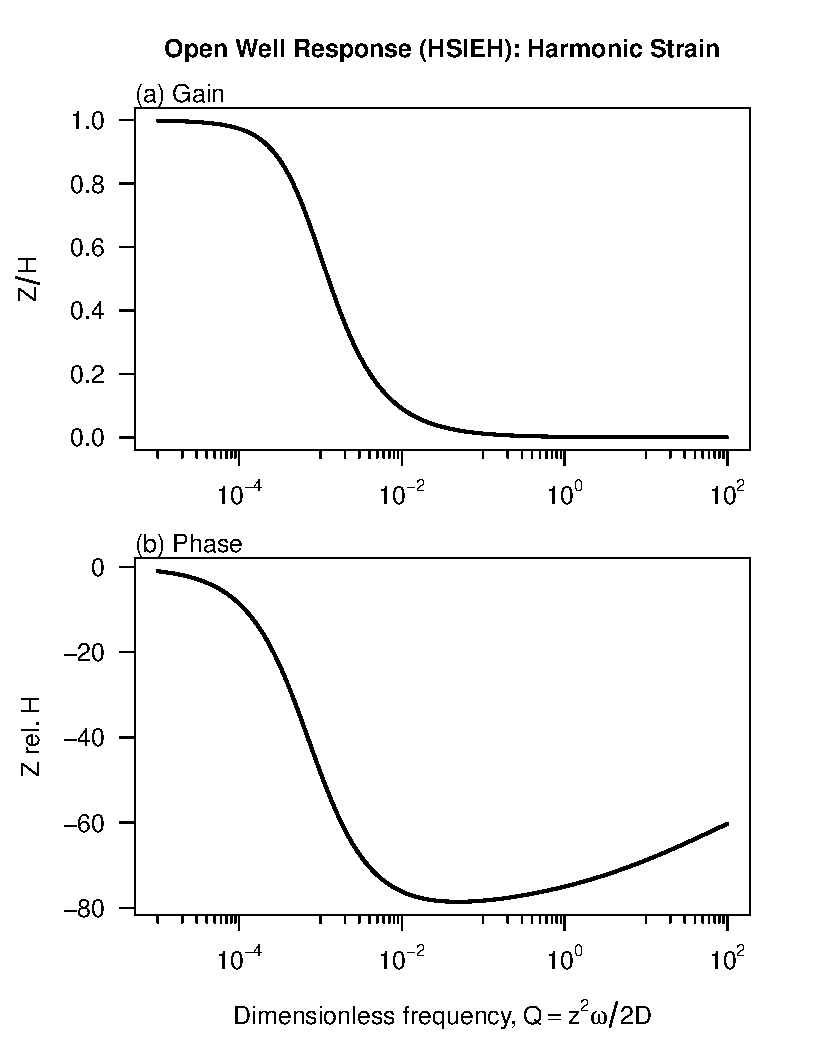
\includegraphics[width=\maxwidth]{figure/HSIEHRESPFIG-1} 

\end{knitrout}
\caption{The response of an open well to harmonic areal strain using
the Hsieh model. 
Frequency is dimensionless, based on the well-depth $z$ and the diffusivity $D$.
}
\label{fig:owrsp-hsi}
\end{center}
\end{figure}

\clearpage
\subsection{Pressure head: Liu et al. (1989)}

\begin{knitrout}\small
\definecolor{shadecolor}{rgb}{0.969, 0.969, 0.969}\color{fgcolor}\begin{kframe}
\begin{alltt}
\hlstd{wrsp} \hlkwb{<-} \hlkwd{open_well_response}\hlstd{(omega,} \hlkwc{T.} \hlstd{= T.,} \hlkwc{S.} \hlstd{= S.,} \hlkwc{Ta} \hlstd{= Ta,} \hlkwc{Hw} \hlstd{= Hw,}
    \hlkwc{model} \hlstd{=} \hlstr{"liu"}\hlstd{,} \hlkwc{as.pressure} \hlstd{= ZasP)}
\hlkwd{plot}\hlstd{(wrsp)}
\end{alltt}
\end{kframe}
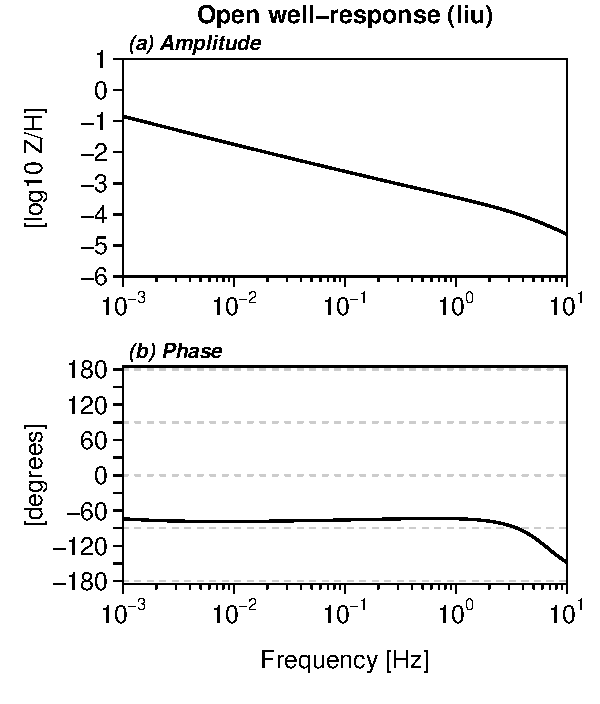
\includegraphics[width=\maxwidth]{figure/LIURESP-1} 
\begin{kframe}\begin{alltt}
\hlstd{crsp} \hlkwb{<-} \hlstd{wrsp[[}\hlstr{"Response"}\hlstd{]][,} \hlnum{2}\hlstd{]}
\hlstd{lGain} \hlkwb{<-} \hlkwd{Mod}\hlstd{(crsp)}
\hlstd{lP} \hlkwb{<-} \hlkwd{Phase}\hlstd{(crsp)}
\end{alltt}
\end{kframe}
\end{knitrout}

\begin{figure}[htb!]
\begin{center}
\begin{knitrout}\small
\definecolor{shadecolor}{rgb}{0.969, 0.969, 0.969}\color{fgcolor}
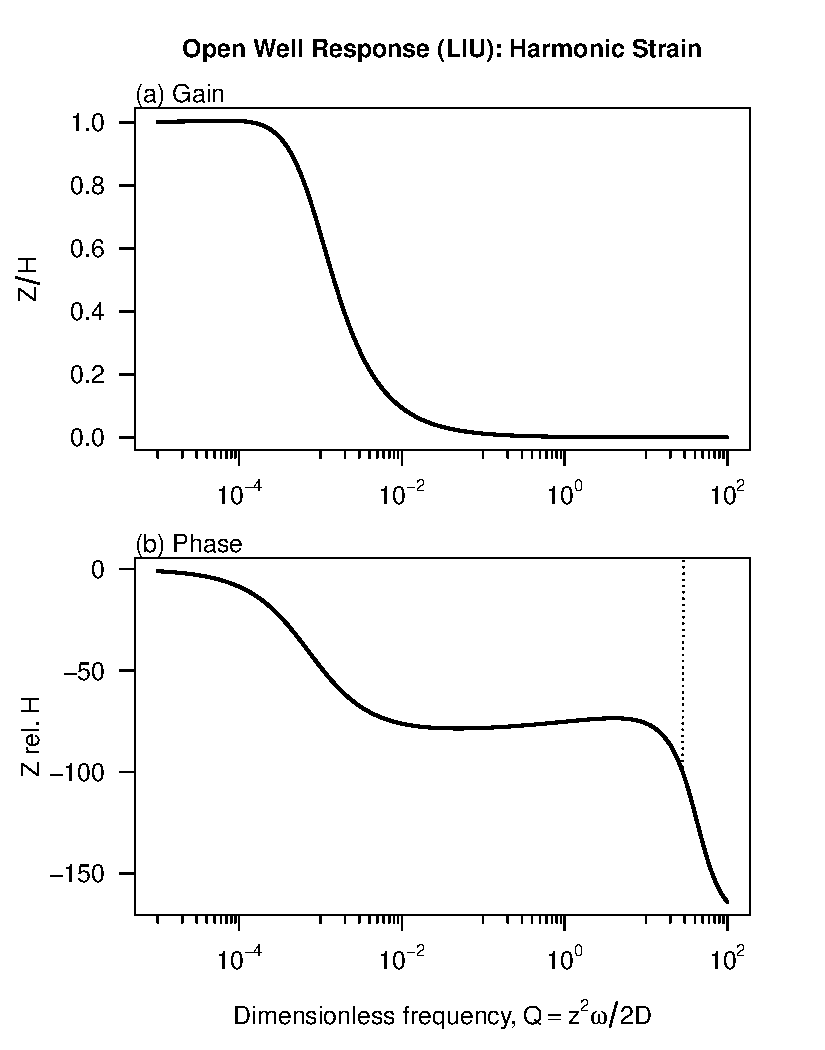
\includegraphics[width=\maxwidth]{figure/LIURESPFIG-1} 

\end{knitrout}
\caption{The response of an open well to harmonic areal strain using
the Liu model. 
Frequency is dimensionless, based on the well-depth $z$ and the diffusivity $D$.
}
\label{fig:owrsp-liu}
\end{center}
\end{figure}

\clearpage
\subsection{Strain: Rojstaczer (1988)}

\begin{knitrout}\small
\definecolor{shadecolor}{rgb}{0.969, 0.969, 0.969}\color{fgcolor}\begin{kframe}
\begin{alltt}
\hlstd{wrsp} \hlkwb{<-} \hlkwd{open_well_response}\hlstd{(omega,} \hlkwc{T.} \hlstd{= T.,} \hlkwc{S.} \hlstd{= S.,} \hlkwc{z} \hlstd{= z,} \hlkwc{model} \hlstd{=} \hlstr{"rojstaczer"}\hlstd{,}
    \hlkwc{as.pressure} \hlstd{= asP)}
\hlkwd{plot}\hlstd{(wrsp)}
\end{alltt}
\end{kframe}
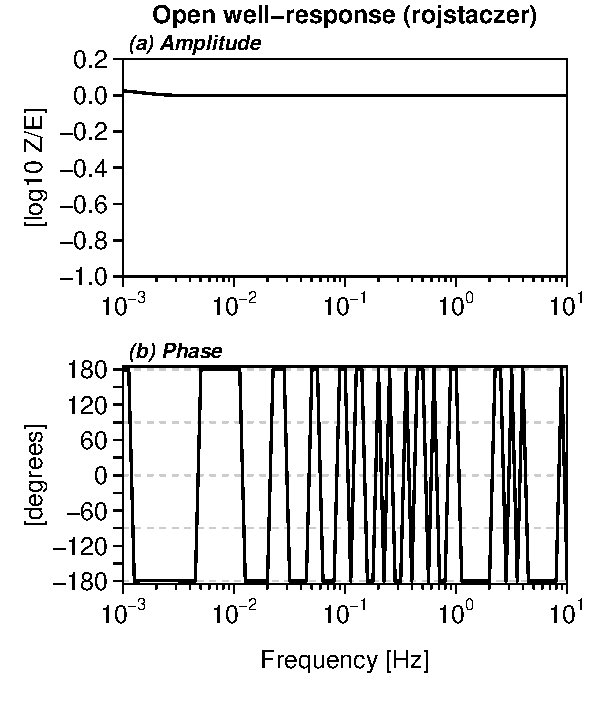
\includegraphics[width=\maxwidth]{figure/ROJRESP-1} 
\begin{kframe}\begin{alltt}
\hlstd{crsp} \hlkwb{<-} \hlstd{wrsp[[}\hlstr{"Response"}\hlstd{]][,} \hlnum{2}\hlstd{]}
\hlstd{rGain} \hlkwb{<-} \hlkwd{Mod}\hlstd{(crsp)}
\hlstd{rP} \hlkwb{<-} \hlkwd{Phase}\hlstd{(crsp)}
\end{alltt}
\end{kframe}
\end{knitrout}

\begin{figure}[htb!]
\begin{center}
\begin{knitrout}\small
\definecolor{shadecolor}{rgb}{0.969, 0.969, 0.969}\color{fgcolor}
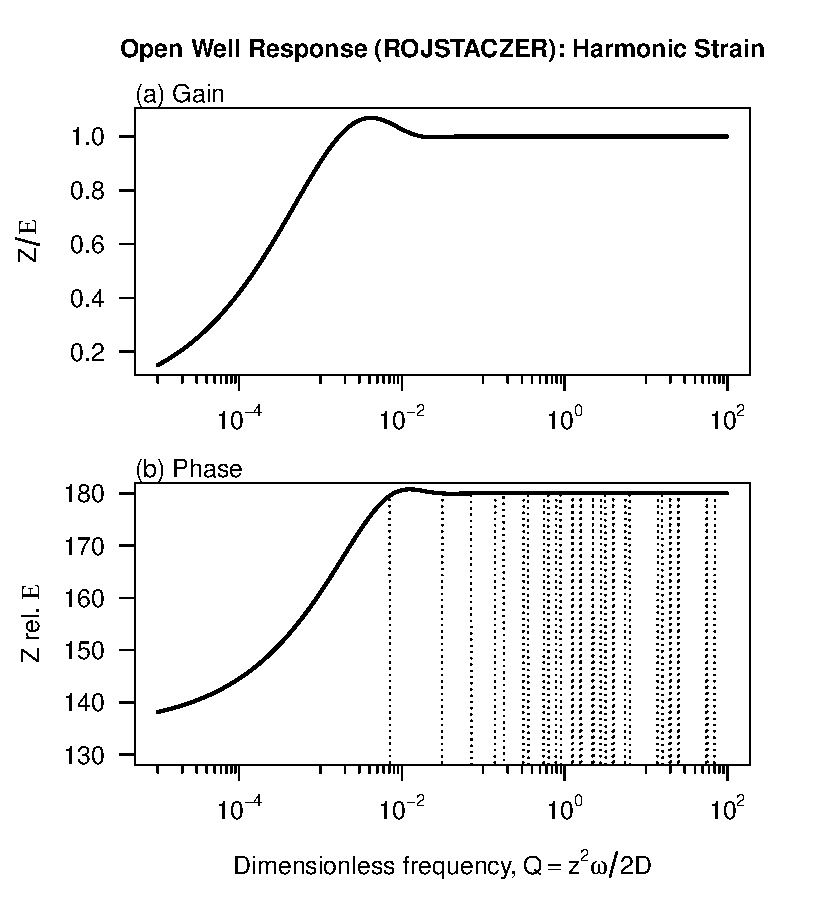
\includegraphics[width=\maxwidth]{figure/ROJRESPFIG-1} 

\end{knitrout}
\caption{The response of an open well to harmonic areal strain using
the Rojstaczer model. Modified from \citet[][Fig.~3]{rojstaczer1988}.
Frequency is dimensionless, based on the well-depth $z$ and the diffusivity
$D$.}
\label{fig:owrsp-roj}
\end{center}
\end{figure}

\clearpage
\section{Model Comparisons}

\subsection{Responses to strain}
\begin{figure}[htb!]
\begin{center}
\begin{knitrout}\small
\definecolor{shadecolor}{rgb}{0.969, 0.969, 0.969}\color{fgcolor}
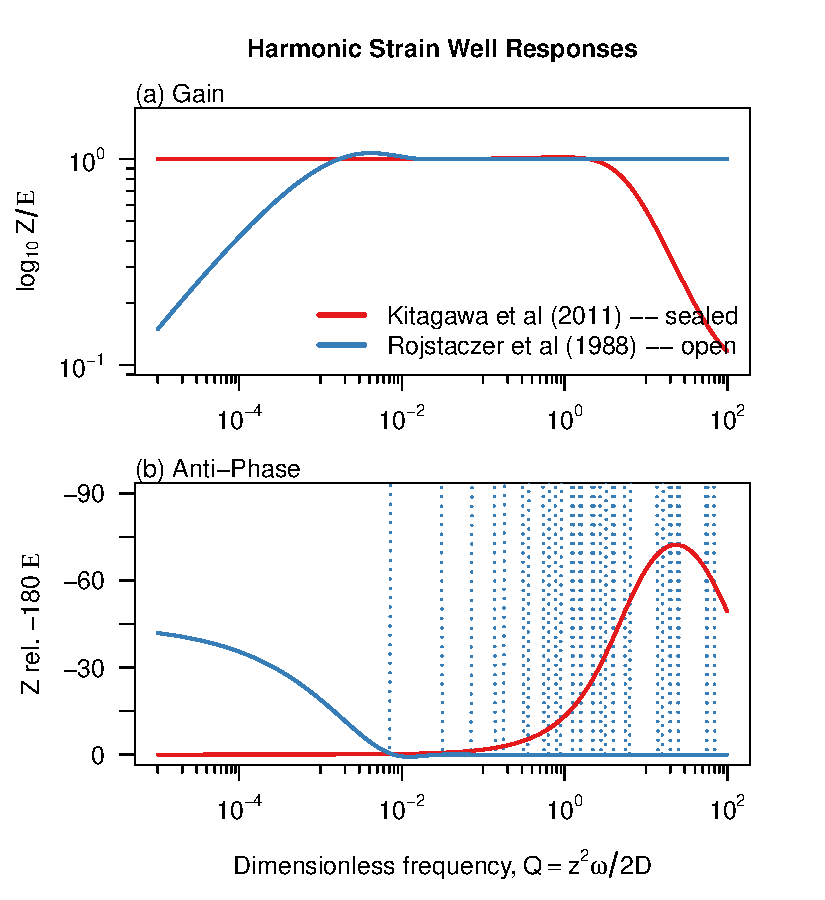
\includegraphics[width=\maxwidth]{figure/ALLRESPFIG-1} 

\end{knitrout}
\caption{A comparison of well responses to harmonic strain. 
The phase of the water level is relative to $-180^\circ$ the phase of strain.}
\label{fig:ewrsp-all}
\end{center}
\end{figure}

\clearpage
\subsection{Responses to pressure head (all open)}
\begin{figure}[htb!]
\begin{center}
\begin{knitrout}\small
\definecolor{shadecolor}{rgb}{0.969, 0.969, 0.969}\color{fgcolor}
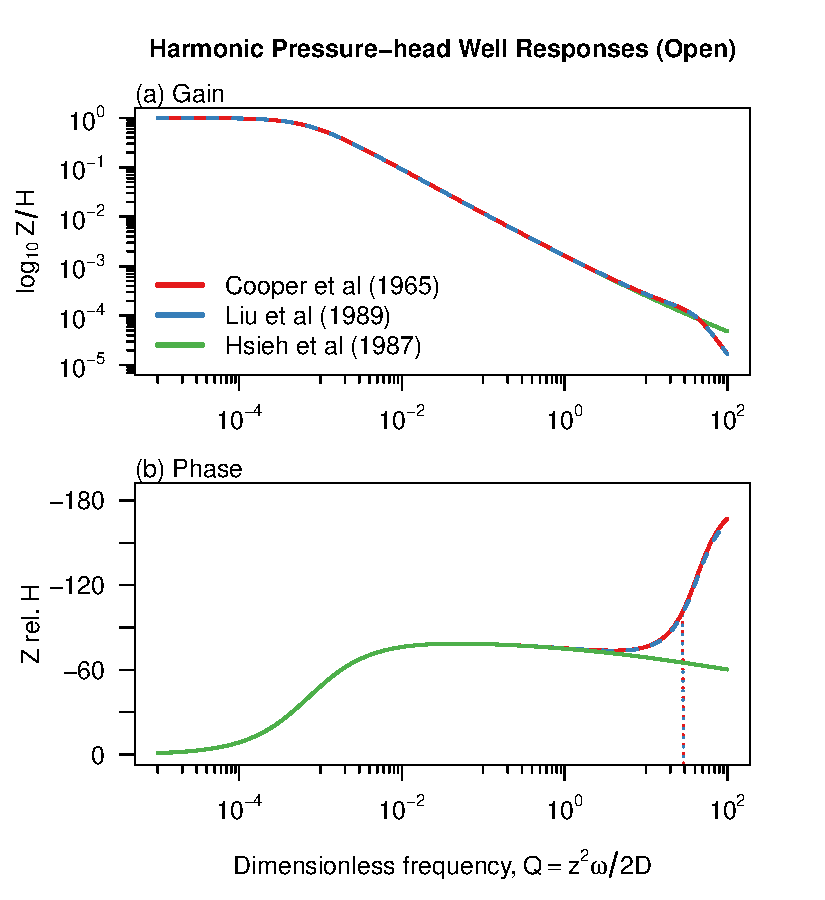
\includegraphics[width=\maxwidth]{figure/ALLORESPFIG-1} 

\end{knitrout}
\caption{A comparison of well responses to harmonic pressure-head, 
from \citet{cooper1965, hsieh1987, liu1989} (all for unsealed).}
\label{fig:owrsp-all}
\end{center}
\end{figure}

\bibliographystyle{apalike}
\bibliography{REFS}

\end{document}
